
\chapter{Introducción}

\chapter{Práctica 1. Manejo básico de Lego Mindstorms NXT: Sensores y Actuadores}

\section{Objetivos}

Tras la realización de esta práctica el alumno debería ser capaz de:
\begin{itemize}
	\item Programar movimientos sincronizados del robot. 
	\item Conocer los parámetros de funcionamiento básico de los motores. 
	\item Utilización  de los sensores básicos. 
\end{itemize}

\section{Ejercicio A}
Calibrar la potencia relativa de los motores para realizar un movimiento lineal con un error menor a 1cm. de desvío por cada 1 m. de avance lineal. (Error menor al 1\%).

\section{Ejercicio B}

\par Programar una maniobra de aparcamiento del robot sin tener en cuenta sensores. Se muestra una descripción del entorno de aparcamiento (Figura~\ref{aparcamiento}). El robot se posicionará con las ruedas motrices rozando la línea lateral y con las ruedas justo por delante de la línea de inicio.

\begin{figure}[ht!]
 \centering
 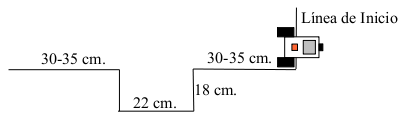
\includegraphics[scale=0.7]{./img/recorrido1.png}
 \caption{Diagrama del aparcamiento.}
 \label{aparcamiento}
\end{figure}


\section{Ejercicio C}

\par Realizar un movimiento de avance del robot teniendo en cuenta los sensores de ultrasonidos y de pulsación, 
que estarán colocados en el frontal de avance del robot. El robot avanzará a plena potencia hasta que se encuentre 
a 1 m. de un obstáculo, que reducirá su potencia a la mitad. A 20 cm. de distancia del obstáculo, el robot reducirá 
su potencia de avance a un cuarto. El avance continuará hasta que el choque sea detectado por el sensor de pulsación, 
en cuyo caso, el robot retrocederá durante 1 seg. y girará 90º a la derecha, comenzando de nuevo el mismo procedimiento.




\chapter{Práctica 2. Manejo básico de Lego Mindstorms NXT: Tareas y Comunicaciones}

\chapter{Práctica 3. Manejo avanzado de Lego Mindstorms NXT}